% !TeX root = ../../thesis.tex
\chapter{Theoretical Background}\label{ch:theory}

\section{Self Consistent Field Methods} \label{sec:SCF}
The objective of any quantum chemical calculation is to solve the time-independent Schrödinger equation (TISE) for a many-electron system:
\begin{equation}\label{eq:TISE}
    \hat{H} \Psi = E \Psi
\end{equation}
However, solving the TISE exactly for systems with more than one electron is computationally infeasible due to the complexity of electron-electron interactions. To address this, approximate methods such as the Hartree-Fock (HF) method have been developed\cite{szabo1996modern}.

The Hartree-Fock (HF) method stands as the cornestone electronic structure calculations. Its primary objective is to provide an approximate solution to the many-electron time-independent Schrödinger equation within the Born-Openhaimer approximation, which governs the behavior of electrons within atoms and molecules:
The HF method achieves this by assuming that each electron moves independently within an average electrostatic field generated by the other electrons in the system. In the HF method the \textit{N}-electron wavefunction is represented by a Slater determinant, which is formed by taking the antisymmetrized product of N individual one-electron spin-orbitals ($\chi$):
\begin{equation}\label{eq:SlaterDet}
    \Psi(\mathbf{r}_1, \mathbf{r}_2, \dots, \mathbf{r}_N) = \frac{1}{\sqrt{N!}}
    \begin{vmatrix}
      \chi_1(\mathbf{r}_1) & \chi_2(\mathbf{r}_1) & \cdots & \chi_N(\mathbf{r}_1) \\
      \chi_1(\mathbf{r}_2) & \chi_2(\mathbf{r}_2) & \cdots & \chi_N(\mathbf{r}_2) \\
      \vdots & \vdots & \ddots & \vdots \\
      \chi_1(\mathbf{r}_N) & \chi_2(\mathbf{r}_N) & \cdots & \chi_N(\mathbf{r}_N)
    \end{vmatrix}
  \end{equation}
The choice of using a deteminant inherently satisfies both the Pauli exclusion principle, and the antisymmetry requirement of fermions. The energy expectation for a Slater determinant according to HF is variational and can be computed as:
\begin{equation}\label{EHF}
    \begin{aligned}
        E_{HF} &= \langle \Psi | \sum_{i=1}^{N} \hat{F}_i  | \Psi \rangle \\
            &= \langle \Psi | \sum_{i=1}^{N} \hat{h}(i) + \sum_{i,j=1}^{N} (2\hat{J}_j(i) - \hat{K}_j(i)) | \Psi \rangle\\ 
            &= \sum_{i=1}^{N} \langle \chi_i | \hat{h} | \chi_i \rangle + \frac{1}{2} \sum_{i,j=1}^{N} \langle \chi_i \chi_j || \chi_i \chi_j \rangle
    \end{aligned}
\end{equation}
Where, $\hat{F}$ is the Fock operator. $\hat{F}$ is made up from $\hat{h}$, the one-electron core Hamiltonian operator (kinetic energy and electron-nucleus attraction); $\hat{J}_j(i)$, the Coulomb operator, describing the electrostatic repulsion between electron i and the average charge distribution of electron j, and $\hat{K}_j(i)$ is the exchange operator, a purely quantum mechanical term arising from the antisymmetry principle. Because of the two electron terms, the computational cost of HF scales as $O(N^4)$. \\
The Hartree-Fock equations are inherently non-linear: because the Fock operator depends on the wavefunctions of all the other electrons, their interactions are coupled. Consequently, these equations cannot be solved analytically and are solved using an iterative procedure known as the self-consistent field (SCF) method, where the final field experienced by the electrons must be consistent with the electron distribution that generates that field. The SCF procedure involves the following steps: An initial guess for the spin-orbitals is made. Using this initial guess, the Fock operator is constructed. The Hartree-Fock equations are then solved by diagonalizing the Fock operator to obtain a new set of molecular orbitals and their corresponding energies. This new set of orbitals is compared to the previous set. If the change is below a predefined threshold, the procedure is considered converged, and the SCF is achieved. If convergence is not reached, the new set of orbitals is used to construct a new Fock operator, and the process is repeated. Convergence signifies that a stable electronic configuration has been reached within the limitations of the Hartree-Fock approximation.\\
In practical Hartree-Fock calculations, the spinorbitals are expressed as linear combinations of predefined mathematical functions known as basis functions. The set of these functions is called a basis set. Because a finite basis set cannot exactly represent the spinorbitals, they greatly define the level of accuracy and computational cost of the calculation. Larger basis sets generally lead to more accurate descriptions of the electronic structure at the cost of increased computational effort.

\subsection{Electron Correlation}
\label{subsec:electron_correlation}
The Hartree-Fock (HF) method is inherently limited by its neglect of the instantaneous interactions of electrons. In the HF approximation, each electron is treated as moving independently within a static, average field created by the other electrons. This mean-field approach fails to account for the fact that electrons will instantaneously repel each other, leading to a correlated movements as they try to avoid each other in space.\\
The primary consequence of neglecting electron correlation in the HF approximation is an overestimation of the electron-electron repulsion energy. While the HF method does account for the exchange interaction exactly as a consequence of the antisymmetry of the Slater determinant (Fermi correlation), it completely neglects the Coulomb, or dynamic, correlation. This omission leads to a higher electronic energy than the exact solution, and an inability to accurately predict certain phenomena, such as London dispersion forces.\\
The difference between the exact non-relativistic energy of the system and the energy obtained in the HF complete basis limit is defined as the correlation energy and is always negative due to the variational principle. Correlated methods aim to include the effects of the instantaneous interactions between electrons that are neglected in the mean-field approximation of HF theory. In the following sections, several correlated methods relevant to this work are presented.

\subsection{Møller-Plesset Perturbation Theory}
Møller-Plesset (MP) perturbation theory offers a way to improve upon the HF energy by the use of Raylei-Schro perturbation theory: the electron correlation is treated as a perturbation to the HF Hamiltonian. The energy and wavefunction are then expanded as a series in terms of the perturbation strength. The first-order energy correction in MP theory is zero, so the first non-trivial correction to the HF energy appears at the second order, giving rise to the MP2 method. The MP2 energy correction for a closed-shell molecule is given by:
\begin{equation} \label{eq:MP2}
    E_{\mathrm{MP2}} = - \frac{1}{4} \sum_{ij}^{\mathrm{occ}} \sum_{ab}^{\mathrm{virt}} \frac{|\langle i j || a b \rangle|^2}{\epsilon_a + \epsilon_b - \epsilon_i - \epsilon_j}
\end{equation}
Where $i,j$ denote occupied molecular orbitals, $a,b$ denote virtual molecular orbitals, and $\epsilon$ are the corresponding orbital energies from the HF calculation. MP theory can be extended to higher orders (MP3, MP4, etc.) to achieve greater accuracy, although the computational cost increases significantly with each order. The computational cost of MP2 scales as $O(N^5)$.

\subsection{Density Functional Theory}
Density Functional Theory (DFT) provides an alternative approach to incorporating electron correlation by parametrizing the energy on the electron density rather than the wavefunction, reducing the degrees of freedom of the system from $3N-3$ to just $3$. In the most commonly used form of DFT, the Kohn-Sham method, the prpblem is formulated terms of orbitals that are not physical, but are chosen to reproduce the electron density of the system. The fundamental principle of DFT is that the ground state energy of a system is a unique functional of its electron density:
\begin{equation}\label{eq:KSDFT}
    \left( -\frac{1}{2} \nabla^2 + \hat{V}_{\mathrm{ext}}(\mathbf{r}) + \hat{V}_\mathrm{H}(\mathbf{r}) + \hat{V}_{\mathrm{XC}}[\rho(\mathbf{r})] \right) \psi_i(\mathbf{r}) = \epsilon_i \psi_i(\mathbf{r})
\end{equation}
Where $\hat{V}_{\mathrm{ext}}$ respresents the external potential, $\hat{V}_\mathrm{H}(\mathbf{r}) = \int \frac{\rho(\mathbf{r}')}{|\mathbf{r} - \mathbf{r}'|} d\mathbf{r}'$ is the Hartree potential, $\hat{V}_{\mathrm{XC}}$ is the Exchange-Correlation potential and $\rho(\mathbf{r})$ is the electron density. The exchange-correlation functional is the most challenging part of DFT, as it is not known exactly and must be approximated. The accuracy of DFT calculations depends heavily on the choice of exchange-correlation functional. The computational cost of DFT scales as $O(N^4)$.

\subsection{Configuration Interaction}
Configuration Interaction (CI) methods improve upon HF by expressing the electronic wavefunction as a linear combination of the HF ground state determinant and excited state determinants:
\begin{equation} \label{eq:CI}
     |\Psi_{\mathrm{CI}} \rangle = c_0 |\Phi_0 \rangle + \sum_{ia} c_{ia} |\Phi_{ia} \rangle + \sum_{ijab} c_{ijab} |\Phi_{ijab} \rangle + \dots
\end{equation}
Where $|\Phi_0 \rangle$ is the HF ground state determinant, $|\Phi_{ia} \rangle$ represents a determinant with a hole in spin-orbital \textit{i} and a particle in the spin-orbital \textit{a}, and c are the CI coefficients. Full CI (FCI),  includes all possible excitations within a given one-electron basis set and represents the exact solution to the non-relativistic Schrödinger equation in that basis. However, is computationally prohibitive for all but the simplest systems. Full Configuration Interaction (FCI) includes all possible excitations within a given one-electron basis set and represents the exact solution to the non-relativistic Schrödinger equation in that basis. However, it is computationally prohibitive for all but the simplest systems.\\ Truncated CI methods, such as CISD (singles and doubles), are more practical but lack size extensivity ---a property ensuring that the energy of a system scales correctly with the number of non-interacting subsystems. A method is size-extensive if, for two infinitely separated molecules $A$ and $B$, the total energy satisfies $E(A + B) = E(A) + E(B)$. Truncated CI methods fail to satisfy this condition because they do not include all necessary higher-order excitations, leading to an underestimation of the total energy as system size grows.\\
CI are, however, size-consistent, meaning that the energy behaviour remains consistent when interaction between the involved molecular subsystems is nullified (by distance, for instance). While CISD is size-consistent, its lack of size extensivity makes it unsuitable for extensive systems.

\subsection{Coupled Cluster Theory} \label{sec:CCTheory}
Similarly to CI, the coupled cluster CC method expands the wavefunction as a linear combination of Slater determinats. However, the CC wavefunction is size-extensive and size-consistent by using an exponential ansatz,
\begin{equation}\label{eq:CCWavenfunc}
    | \Psi_{\mathrm{CC}} \rangle = e^{\hat{T}} | \Psi_{0} \rangle
\end{equation}
where $\hat{T}$ is the cluster operator, which is the central component of CC theory and is defined as a sum of excitation operators,
\begin{equation}
    \hat{T} = \hat{T}_1 + \hat{T}_2 + \hat{T}_3 + \dots + \hat{T}_N
\end{equation}
where $N$ is the total number of electrons in the system. Each term in this sum corresponds to a specific level of excitation and is expressed within the second quantization formalism:
\begin{itemize}
    \item $\hat{T}_1 = \sum_{i}^{\text{occ}} \sum_{a}^{\text{virt}} t_i^a a_a^{\dagger} a_i$ represents single excitations.
    \item $\hat{T}_2 = \frac{1}{4} \sum_{i,j}^{\text{occ}} \sum_{a,b}^{\text{virt}} t_{ij}^{ab} a_a^{\dagger} a_b^{\dagger} a_j a_i$ represents double, \textit{coupled} excitations.
    \item Higher-order excitation operators $\hat{T}_3, \hat{T}_4, \dots$ describe coupled excitation of three, four, and more electrons, respectively.
\end{itemize}
The coefficients $t_i^a$, $t_{ij}^{ab}$, etc., are cluster amplitudes to determined by projection of the CC Schr\"{o}dinger equation onto the excited determinant. The exponential form, expanded as a Taylor series,
\begin{equation}
    e^{\hat{T}} = 1 + \hat{T} + \frac{1}{2!} \hat{T}^2 + \dots
\end{equation}
inherently includes terms that represent disconnected clusters, which are ensures for size consistency. The energy is obtained by projecting onto the HF reference determinant:
\begin{equation}\label{eq:CCEnergy}
    E_{\mathrm{CC}}=\langle \Psi_{0} | e^{-\hat{T}} \hat{H} e^{\hat{T}} | \Psi_{0} \rangle
\end{equation}
Using the Baker-Campbell-Hausdorff expansion, the exponential operators in Eq. \ref{eq:CCEnergy} can be simplified to a series of commutators which ends at the fourth order. The cluster operator $\hat{T}$ can be truncated at different levels of excitation:
\begin{itemize}
    \item \textbf{CCD} (Coupled Cluster Doubles): This is the simplest approximation in the CC family, where the cluster operator is truncated to include only double excitations: $\hat{T} \approx \hat{T}_2$. There is no CC Singles since the Brilluin's theorem implies that the amplitudes of single excitations alone are null. 
    \item \textbf{CCSD} (Coupled Cluster Singles and Doubles): This is one of the most widely used and generally accurate \textit{ab initio} methods, where the cluster operator includes both single and double excitations: $\hat{T} \approx \hat{T}_1 + \hat{T}_2$.
    \item \textbf{CCSDT} (Coupled Cluster Singles, Doubles, and Triples): $\hat{T} \approx \hat{T}_1 + \hat{T}_2 + \hat{T}_3$.
    \item \ldots
\end{itemize}
The hierarchy can be extended to include even higher levels of excitation,  with the properties converging to the FCI limit. The computational cost of CC methods increases rapidly with the level of truncation, as shown in Table \ref{tab:qc_scaling}.
\begin{table}[h!]
    \centering
    \begin{tabular}{ccc}
        Method & Operation count & Memory \\
        \hline
        HF & $O(N^4)$ & $O(N^4)$ \\
        DFT & $O(N^4)$ & $O(N^4)$ \\ 
        MP2 & $O(N^5)$ & $O(N^4)$ \\
        CCD/CCSD & $O(N^6)$ & $O(N^4)$ \\
        CCSDT & $O(N^8)$ & $O(N^6)$ \\
        CC2 & $O(N^{5})$ & $O(N^4)$ \\
    \end{tabular}
    \caption[Computational Scaling of Methods]{Computational scaling of quantum chemistry methods.}
    \label{tab:qc_scaling}
\end{table}

\subsection{Second Approximate Coupled Cluster}\label{sec:CC2Theory}
Second Approximate Coupled Cluster (CC2) belongs to the broader family of CCn approximate coupled cluster methods, where the `n' in CCn indicates the truncation of the cluster operator within a perturbative hierarchy. These methods aim to reduce the computational cost associated with standard CC truncations while still retaining a reasonable level of accuracy.\\

In CC2, the equations for the single amplitudes, $t^a_i$, are the same as CC theory (Eq. \ref{eq:CCWavenfunc}) under the constraint that the doubles amplitudes, $t^{ab}_{ij}$, are calculated using the non-iterative expression for MP2 (Eq \ref{eq:MP2}). The resulting expression for the CC2 correlation energy is:
\begin{equation}\label{CC2Energy}
    E_{\mathrm{CC2}} = \frac{1}{4}\sum_{ij}^{\mathrm{occ}} \sum_{ab}^{\mathrm{virt}} \frac{|\langle i j || a b \rangle|^2}{\epsilon_a + \epsilon_b - \epsilon_i - \epsilon_j}  + \sum_{i}^{\mathrm{occ}} \sum_{a}^{\mathrm{virt}} \hat{F}_{ai} t^a_i 
\end{equation}
The perturbative treatment of the doubles amplitudes in CC2, reduces the computational cost compared to CCSD, Table \ref{tab:qc_scaling}. While this approximation can lead to a less accurate description of electron correlation, the inclusion of singles amplitudes allows for an approximate description of orbital relaxation, which often leads to higher quality wavefunction, and hence properties, compared to MP2.

\section{Equation-of-Motion Methods} \label{sec:eom_theory}
Equation-of-Motion Coupled Cluster (EOM-CC) methods are an extension of ground-state coupled cluster theory which provide a framework for calculating a variety of excited (EE), ionized (IP) and electron-attached (EA) states. In the EOM-CC, the target electronic state is generated by applying a linear excitation operator $\hat{R}$ to a reference state, which typically is the coupled cluster wavefunction of the ground state. The target state wavefunction can then be expressed as $|\Psi_{\mathrm{EOM}}\rangle = \hat{R} |\Psi_{\mathrm{CC}}\rangle = \hat{R} e^{\hat{T}} |\Phi_{\mathrm{HF}}\rangle$. Figure \ref{fig:EOM}, shows some of the determinats of $| \Psi_{\mathrm{EA}} \rangle$, where the target state has one more $\mathrm{\alpha}$ electron. \\

The form of the operator $\hat{R}$ is similar to the cluster operator and chosen to access the desired target state. In the case of EOM-EA, the electron attachment operator $R^{\text{EA}}$ includes terms that describe the creation of one electron to an unoccupied orbital, terms that describe the creation of one electron accompanied by the excitation of another electron from an occupied to an unoccupied orbital, and so on:
\begin{equation}\label{eq:R_EA}
    \hat{R}^{\mathrm{EA}} = \hat{R}_1^{\mathrm{EA}} + \hat{R}_2^{\mathrm{EA}} + \ldots = \sum_{a} r^a a_a^{\dagger} + \frac{1}{2}\sum_{ab} \sum_{i} r^{ba}_{i} a_b^{\dagger} a_a^{\dagger} a_i + \ldots
\end{equation}
\begin{figure}
    \centering
    \medskip
    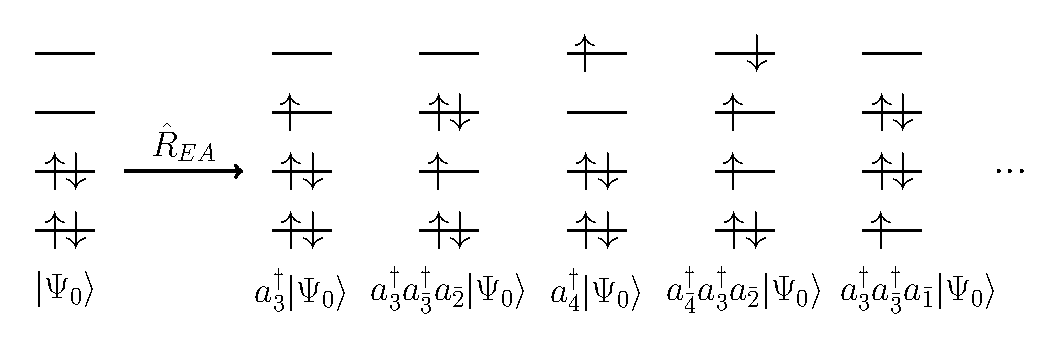
\includegraphics[width=.8\textwidth]{EOM_EA}
    \caption{EOM-EA.}
    \label{fig:EOM}
  \end{figure}
  Where $a$ and $b$ denote virtual orbitals, $i$ denotes an occupied orbital, and $r^a$ and $r^{ba}_{i}$ are the coefficients to be determined. By truncating at the same excitation level as the cluster operator, the method is rigorously size-extensive and size-consistent. The EA energies, or any other EOM energy, can be obtained as the eigenvalues of the similarity-transformed Hamiltonian, $\bar{H}_{\mathrm{N}}$:
\begin{equation}
    \bar{H}_{\mathrm{N}} \hat{R} | \Psi_0 \rangle = \Delta E_{\mathrm{EOM}} \hat{R} | \Psi_0 \rangle
\end{equation}
\begin{equation}
    \bar{H}_{\mathrm{N}} = e^{-\hat{T}} \hat{H} e^{\hat{T}} - \langle \Psi_0 | e^{-\hat{T}} \hat{H} e^{\hat{T}} | \Psi_0 \rangle
\end{equation}
Since the similarity trnasformed hamiltonian is non-hermitian, the left and right are different but correspond to the same eigenvalues. This means that the properties have `right' and `left' expectation values. \\
The strength of the EOM-CC ansatz is the use of a closed shell reference to access open shell states, which are eigenfunctions of the $\hat{S}^2$ operator. The EOM-CC methods are also size-extensive and size-consistent. The computational cost of EOM-CC methods is similar to that of the corresponding ground-state CC methods.

\section{Dyson Orbitals}

Dyson orbitals are defined as the overlap between the wavefunction of an initial $N$-electron state ($|\Psi_0^N\rangle$) and the wavefunction of the final state with $N\pm1$ electrons ($|\Psi_f^{N\pm1}\rangle$).
\begin{equation}
    \phi_{d}(r_1) = \sqrt{N} \int \Psi^{N}(r_2,\dots,r_N) \Psi^{N+1}(r_1, r_2,\dots,r_N)\,dr_2 \dots dr_N
\end{equation}
Because the the terms differ in one electron, the result of the overlap is a vector instead of a scalar, and can be expressed as a linear combination of the molecular orbitals ($\phi_p(r)$) of the reference wavefunction:
\begin{equation}
    \phi_{d}(r) = \sum_p \gamma_p \phi_p(r)
\end{equation}
where $\gamma_p$ are the coefficients that quantify the contribution of each molecular orbital to the Dyson orbital. Physically, Dyson orbitals can be interpreted as the correlated analog to the orbital of the electron that is either removed or attached.

The norm squared of the Dyson orbital, ($P$), is calculated by integrating the squared modulus of the Dyson orbital over all space:
\begin{equation}
    P = \int |\phi_{Dyson}(r)|^2 \,dr = \sum_{p,q} \gamma_p^* \gamma_q \langle \phi_p | \phi_q \rangle
\end{equation}
The pole strength ranges from 0 to 1 and provides a direct measure of the one-electron character of the ionization or electron attachment process. As the open shell wavefunction is usually obtained by means of a EOM-CC method, there are a `left' and `right' Dyson orbital.


They can be used for the interpretation and prediction of photoelectron spectra as they contain all the information required to calculate diffrential corss-sections, $\frac{d\sigma}{d\Omega_k}$:
\begin{equation}
    \frac{d\sigma}{d\Omega_k} = \frac{4\pi^2kE}{c}|\langle \phi_d | \mu | \Psi^{el}_k \rangle |^2
\end{equation}
where where \textit{k} is the magnitude of the photoelectron wavevector, \textit{E} is the energy of the ionizing radiation, and \textit{c} is the speed of light, $\mu$ is the dipole operator, and $\Psi^{el}_k$ is the photoelectron wavefunction, and a strong orthonormality is assumed between the reference and continuum wavefunction.  

\subsection{EOM-CC2 Dyson Orbital Equations\label{sec:theory_dyson}}
Justify that the expression doesnt change from CCSD (see TJ email).\\

\subsubsection{EOM-EA-Dyson Equations}
A derivation of the algebraic expression of Dyson orbitals in terms of the $t,\, r,\, l,\, \lambda$ amplitudes is presented.
It is importnat to realize that the operators involved ($\hat{T},\hat{\Lambda},\hat{R},\hat{L}$) affect the occupation of the spin-orbitals, and thus only the combinations of terms which leave the refrence wavefunction, $| 0 \rangle$, unchanged survive. To find these combinations, commutators can be used to reorder the operators involved:

In the case of the right EOM-EA-Dyson orbital amplitudes:
 \[\gamma^\mathrm{EA,R}_{i} = \langle EA | \hat{a}^{\dagger}_i | CC \rangle =  \langle 0|\hat{L}^{EA} e^{-\hat{T}} \hat{a}^{\dagger}_i e^{\hat{T}} | 0 \rangle \]
 The following equalities are usueful:
\[
e^{-{\hat{T}}}e^{{\hat{T}}}=e^{{\hat{T}}}e^{-{\hat{T}}}=1 \]\[
[e^{\pm{\hat{T}}},\hat{a}^{\dagger}_p]=\cancelto{0}{[1,\hat{p}^{\dagger}]} \pm t^b_j[\hat{b}^{\dagger}\hat{j},\hat{p}^{\dagger}] \pm t^{bc}_{jk}[\hat{b}^{\dagger}\hat{c}^{\dagger}\hat{k}\hat{j},\hat{p}^{\dagger}] + \ldots
\]
Where a change of notation, $a^\dagger_p \rightarrow p^\dagger$, upon expansion is done for readibility. Two cases are distinguished, $p$ is a virtual orbital, $a$, or an occupied orbital, $i$.
For virtual orbitals, $p=a$:
\[
[\hat{b}^{\dagger}\hat{j},\hat{a}^{\dagger}] = \hat{b}^{\dagger}\hat{j}\hat{a}^{\dagger} - 
\hat{a}^{\dagger}\hat{b}^{\dagger}\hat{j} = (-1)^2\hat{a}^{\dagger}\hat{b}^{\dagger}\hat{j} - 
\hat{a}^{\dagger}\hat{b}^{\dagger}\hat{j} = 0 \] Similarly with higher order terms, it is arribed to:
\[
[e^{\pm {\hat{T}}},\hat{a}^{\dagger}_a] = 0 
\]
For occupied orbitals, $p=i$:
\[
[\hat{b}^{\dagger}\hat{j},\hat{i}^{\dagger}] = \hat{b}^{\dagger}\hat{j}\cancelto{0}{\hat{i}^{\dagger}} - 
\hat{i}^{\dagger}\hat{b}^{\dagger}\hat{j} \] And similarly with higher order terms:
\[
[e^{\pm {\hat{T}}},\hat{a}^{\dagger}_i] = -\hat{a}^{\dagger}_i(e^{\pm {\hat{T}}}-1) 
\]
These relations can now be used to derive the expression for the occupied and virtual Right EOM-EA-Dyson orbital amplitudes: \[ \phi^\mathrm{EA,R}_\mathrm{D} = \sum_p^\mathrm{} \gamma^\mathrm{EA,R}_p \phi_p= \sum_i^\mathrm{occ} \gamma^\mathrm{EA,R}_i \phi_i + \sum_a^\mathrm{vir} \gamma^\mathrm{EA,R}_a \phi_a \]
The general expression can be reordered:
\noindent\begin{flalign}
   \qquad  \gamma^\mathrm{EA,R}_{p} &= \langle EA | \hat{a}^{\dagger}_p | CC \rangle =  \langle 0|\hat{L}^{EA}e^{-{\hat{T}}}\hat{a}^{\dagger}_p e^{\hat{T}} | 0 \rangle \notag &\\
    & = \langle 0|\hat{L}^{EA}(\hat{a}^{\dagger}_p e^{-{\hat{T}}} + [e^{-{\hat{T}}},\hat{a}^{\dagger}_p]) e^{\hat{T}} | 0 \rangle
\end{flalign}
For virtual orbitals, $p=a$:
\noindent\begin{flalign}
    \qquad \gamma^\mathrm{EA,R}_{a} &= \langle 0|\hat{L}^{EA}(\hat{a}^{\dagger}_a e^{-{\hat{T}}} + \cancelto{0}{[e^{-{\hat{T}}},\hat{a}^{\dagger}_a]}) e^{\hat{T}} | 0 \rangle \notag &\\
    & = \langle 0|\hat{L}^{EA}\hat{a}^{\dagger}_a\, \cancelto{1}{e^{-{\hat{T}}}e^{\hat{T}}} | 0 \rangle = \langle 0|\hat{L}^{EA}\hat{a}^{\dagger}_a | 0 \rangle \notag &\\
    & = \langle 0| l_a \hat{a} \hat{a}^\dagger | 0 \rangle \notag &\\
    & = l_a
\end{flalign}
For occupied orbitals, $p=i$:
\noindent\begin{flalign}
    \qquad \gamma^\mathrm{EA,R}_{i} &= \langle 0|\hat{L}^{EA}(\hat{a}^{\dagger}_i e^{-{\hat{T}}} + [e^{-{\hat{T}}},\hat{a}^{\dagger}_i]) e^{\hat{T}} | 0 \rangle \notag &\\
    & = \langle 0 | \hat{L}^{EA}(\cancelto{0}{\hat{a}^{\dagger}_i e^{-{\hat{T}}} -\hat{a}^{\dagger}_ie^{-{\hat{T}}}} + \hat{a}^{\dagger}) e^{\hat{T}} | 0 \rangle = \langle 0 | \hat{L}^{EA} \hat{a}^{\dagger}_i e^{\hat{T}} | 0 \rangle  \notag &\\
    & = \langle 0 | l_b t_i^b \, \hat{b} \hat{i}^{\dagger} \hat{b}^{\dagger}\hat{i}+ l_{bc}^j t_{ij}^{bc} \, \hat{b}\hat{c}\hat{j}^{\dagger}\hat{i}^{\dagger}\hat{b}^{\dagger}\hat{c}^{\dagger}\hat{i}\hat{j} | 0 \rangle  \notag &\\ 
    &  = - \sum_c t_{ic} l_c - \frac{1}{2} \sum_{kcd} t_{ki}^{dc} l_{dc}^k
\end{flalign}
A similar approach can be applyed to the other Dyson equations to obtain the expressions.
\iffalse
Right Dyson orbital, $ \phi^\mathrm{EA,R}_\mathrm{D} = \sum_i^\mathrm{occ} \gamma^\mathrm{EA,R}_i \phi_i + \sum_a^\mathrm{vir} \gamma^\mathrm{EA,R}_a \phi_a $:
\noindent\begin{flalign}
   \qquad  \gamma^\mathrm{EA,R}_{i} &= \langle EA | \hat{a}^{\dagger}_i | CC \rangle =  \langle 0|\hat{L}^{EA}\hat{a}^{\dagger}_i e^{\hat{T}} | 0 \rangle \notag &\\
    &  = - \sum_c t_{ic} l_c - \frac{1}{2} \sum_{kcd} t_{ki}^{dc} l_{dc}^k \\
     \gamma^\mathrm{EA,R}_{a}&= \langle EA | \hat{a}^{\dagger}_a | CC \rangle \notag \\
    & = l_a
\end{flalign}\fi

Left EOM-EA-Dyson orbital, $ \phi^\mathrm{EA,L}_\mathrm{D} = \sum_i^\mathrm{occ} \gamma^\mathrm{EA,L}_i \phi_i + \sum_a^\mathrm{vir} \gamma^\mathrm{EA,L}_a \phi_a$:
\noindent\begin{flalign}
    \qquad \gamma^\mathrm{EA,L}_{i} &= \langle CC | \hat{a}_i | EA \rangle \notag & \\ 
    & = - \sum_c \lambda_{ic} r_{c} - \frac{1}{2} \sum_{kcd} \lambda_{ik}^{cd} r_{k}^{dc} \\
    \gamma^\mathrm{EA,L}_{a} &= \langle CC | \hat{a}_a | EA \rangle \notag \\
    & = r_a + \sum_{kc} \lambda_{kc} r_{ca}^k + \sum_k \gamma^\mathrm{EA,L}_k t_{ka} - \frac{1}{2} \sum_{klcd} \lambda_{lk}^{dc} t_{lk}^{da} r_{c}
\end{flalign}

\subsubsection{EOM-EA-EE-Dyson Equations}
Right Dyson orbital, $ \phi^\mathrm{EA-EE,R}_\mathrm{D} = \sum_i^\mathrm{occ} \gamma^\mathrm{EA-EE,R}_i \phi_i + \sum_a^\mathrm{vir} \gamma^\mathrm{EA-EE,R}_a \phi_a $:

\noindent\begin{flalign}
    \qquad \gamma^\mathrm{EA-EE,R}_{i} &= \langle EA | \hat{a}^{\dagger}_i | EE \rangle \notag & \\
    & = r_0 \gamma^\mathrm{EA,R}_a - \sum_c r_{ic} l_c - \frac{1}{2} \sum_{lcd} r_{il}^{cd} l_{dc}^l - \sum_{lcd} l_{dc}^l t_{ic} r_{ld} \\
    \gamma^\mathrm{EE-EA,R}_{a} &= \langle EA | \hat{a}^{\dagger}_a | EE \rangle \notag &\\
    & = r_0 l_a + \sum_{kc} l_{ca}^k r_{kc}
\end{flalign}

Left Dyson orbital, $ \phi^\mathrm{EE-EA,L}_\mathrm{D} = \sum_i^\mathrm{occ} \gamma^\mathrm{EE-EA,L}_i \phi_i + \sum_a^\mathrm{vir} \gamma^\mathrm{EE-EA,L}_a \phi_a$:
\noindent\begin{flalign}
    \qquad \gamma^\mathrm{EE-EA,L}_{i} &= \langle EE | \hat{a}_i | EA \rangle \notag & \\
    & = - \sum_c l_{ic}r_{c} - \frac{1}{2} \sum_{kcd} l_{ik}^{cd} r_{k}^{dc} \\ 
    \gamma^\mathrm{EE-EA,L}_{a} &= \langle EE | \hat{a}_a | EA \rangle \notag \\
    & = \sum_{kc} l_{kc}r_{ca}^k + \sum_k \gamma^\mathrm{EE-EA,L}_k t_{ka} - \frac{1}{2} \sum_{klcd} l_{lk}^{dc} t_{lk}^{da} r_{c}
\end{flalign}

\subsubsection{EOM-IP-Dyson Equations}
Right Dyson orbital, $ \phi^\mathrm{EE,R}_\mathrm{D} = \sum_i^\mathrm{occ} \gamma^\mathrm{IP,R}_i \phi_i + \sum_a^\mathrm{vir} \gamma^\mathrm{IP,R}_a \phi_a $:

\noindent\begin{flalign}
    \qquad     \gamma^\mathrm{IP,R}_{a} &= \langle CC | \hat{a}^{\dagger}_a | IP \rangle \notag \\
    &= \lambda_{ka}r_{k} + \frac{1}{2} \lambda_{lk}^{ca} r_{klc} \\
    \gamma^\mathrm{IP,R}_{i} &= \langle CC | \hat{a}^{\dagger}_i | IP \rangle \notag & \\
    &= r_i + \sum_{kc} \lambda_{kc}r_{ik}^c - \sum_c \gamma^\mathrm{IP,R}_c t_{ic} - \frac{1}{2} \sum_{klcd} \lambda_{lk}^{dc} t_{li}^{dc} r_{k}
\end{flalign}

Left Dyson orbital, $ \phi^\mathrm{IP,L}_\mathrm{D} = \sum_i^\mathrm{occ} \gamma^\mathrm{IP,L}_i \phi_i + \sum_a^\mathrm{vir} \gamma^\mathrm{IP,L}_a \phi_a$:
\noindent\begin{flalign}
    \qquad     \gamma^\mathrm{IP,L}_{i} &= \langle IP | \hat{a}_i | CC \rangle \notag \\
    &= l_i \\
    \gamma^\mathrm{IP,L}_{a} &= \langle IP | \hat{a}_a | CC \rangle \notag & \\
    &= \sum_k t_{ka} l_k + \frac{1}{2} \sum_{klc} t_{kl}^{ac} l_{kl}^c
\end{flalign}

\subsubsection{EOM-EE-IP-Dyson Equations}
Right Dyson orbital, $ \phi^\mathrm{EE-IP,R}_\mathrm{D} = \sum_i^\mathrm{occ} \gamma^\mathrm{EE-IP,R}_i \phi_i + \sum_a^\mathrm{vir} \gamma^\mathrm{EE-IP,R}_a \phi_a $:

\noindent\begin{flalign}
    \qquad \gamma^\mathrm{EE-IP,R}_{i} &= \langle EE | \hat{a}^{\dagger}_i | IP \rangle \notag  &\\
    &= \sum_{kc} l_{kc}r_{ik}^c - \sum_c \gamma^{IP-EI}_c t_{ic} - \frac{1}{2} \sum_{klcd} l_{lk}^{dc} t_{li}^{dc} r_{k} \\
    \gamma^\mathrm{EE-IP,R}_{a} &= \langle EE | \hat{a}^{\dagger}_a | IP \rangle \notag \\
    &= l_{ka}r_{k} + \frac{1}{2} l_{lk}^{ca} r_{klc}
\end{flalign}

Left Dyson orbital, $\phi^\mathrm{IP-EE,L}_\mathrm{D} = \sum_i^\mathrm{occ} \gamma^\mathrm{IP-EE,L}_i \phi_i + \sum_a^\mathrm{vir} \gamma^\mathrm{IP-EE,L}_a \phi_a$:
\noindent\begin{flalign}
    \qquad \gamma^\mathrm{IP-EE,L}_{i} &= \langle IP | \hat{a}_i | EE \rangle \notag & \\
    &= r_0 l_i + \sum_{kc} l_{ik}^c r_{kc} \\
    \gamma^\mathrm{IP-EE,L}_{a} &= \langle IP | \hat{a}_a | EE \rangle \notag \\
    &= r_0 \gamma^\mathrm{IP,L}_a + \sum_k r_{ka} l_k + \frac{1}{2} \sum_{klc} r_{kl}^{ac} l_{kl}^c + \sum_{klc} l_{kl}^c t_{ka} r_{cl}
\end{flalign}

%%%%%%%%%%%%%%%%%%%%%%%%%%%%%%%%%%%%%%%%%%%%%%%%%%
% Keep the following \cleardoublepage at the end of this file, 
% otherwise \includeonly includes empty pages.
\cleardoublepage

% vim: tw=70 nocindent expandtab foldmethod=marker foldmarker={{{}{,}{}}}